\subsection{FPGA并行优化方法}
\subsubsection{元件间并行}
ClickNP的模块化架构自然地实现了不同元件之间的并行化,其工具链将元件实例映射到FPGA上的硬件区块,
不同区块间通过先进先出缓冲器连接,因而可以彼此独立地并行工作。
因此,ClickNP配置文件中的每个实例化元件均可视为具有专门功能的独立的核。
网络包以帧为单位在元件之间传播,各级元件可以流水化并行处理。
在单元件处理能力不足时,还可以通过增加元件数,实现数据级并行。
对于网络流量而言,流水线并行和数据并行均可用于加速其处理性能,
且在ClickNP平台上可以灵活地实现这些并行。

\begin{figure}[htbp]
\centering
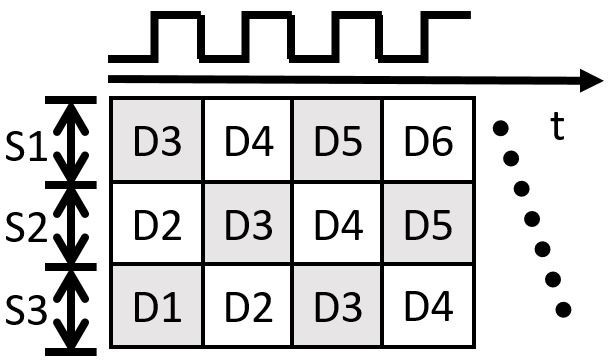
\includegraphics[width=4in]{pipeline}
\caption{多级流水线操作}\label{fig:pipeline}
\end{figure}

\subsubsection{元件内并行}
与逐条执行指令的CPU不同,FPGA通过硬件逻辑执行数据操作。
如果在一个处理函数中需要对单个数据进行多次操作,高级编程工具会将其转化为多级流水线操作。
每一时钟周期,将流水线推进一级,并移进新的数据,如图~\ref{fig:pipeline} 所示。

多级流水线操作可以使处理函数平均每个时钟周期处理完一单位数据,以实现吞吐率最大化。
